%\section{Baseline Methods}
%\label{sec:method}
%In this section, we first formulate the tasks and propose two kinds of baseline methods in the two following sections, feature-based methods and LSTM-based methods.
%
\section{Sentence-level \lnear\ Relation Classification}
\label{sec:classify} 
\textbf{Problem Statement} 
Given a sentence $s$ mentioning a pair of physical objects 
\textless$e_i,e_j$\textgreater, we call \textless$s,e_i,e_j$\textgreater
~an {\em instance}. 
For each instance, the problem is to determine whether $e_i$ and $e_j$ are located near each other in the physical scene described in the sentence $s$.
For example, suppose $e_i$ is ``dog", $e_j$ is ``cat'', and $s$ = ``\textit{The King puts his dog and cat on the table.}''.
As it is true that the two objects are located near in this sentence, a successful classification model is expected to label this instance as \textit{True}.
%and
However, if $s_2$ = ``\textit{My dog is older than her cat.}'', then the label of the instance \textless$s_2,e_i,e_j$\textgreater ~is \textit{False}, because $s_2$ just talks about a comparison in age.
%While the dog and the cat in $s_2$ do not have to be located near \textless$s_2,e_i,e_j$\textgreater ~is \textit{False}.
In the following subsections, we present two different kinds of baseline methods for this binary classification task: feature-based methods and  LSTM-based neural architectures.

\subsection{Feature-based Methods}
\label{sec:feature}
Our first baseline method is an SVM classifier based on following features commonly used in many relation extraction models~\cite{xu2015classifying}: 
\begin{compactenum}
	\item  \textit{Bag of Words (BW)}:
	the set of words that ever appeared in the sentence. 
	\item \textit{Bag of Path Words (BPW)}:
	the set of words that appeared on
	the shortest dependency path between objects $e_i$ and $e_j$ in the 
	dependency tree of the sentence $s$, plus the words in the two subtrees 
	rooted at $e_i$ and $e_j$ in the tree.
	\item \textit{Bag of Adverbs and Prepositions (BAP)}:
	the existence of adverbs and prepositions in the sentence as binary features. 
	\item \textit{Global Features (GF)}:
	the length of the sentence, the number of nouns, verbs, adverbs, adjectives, determiners, prepositions and punctuations in the whole sentence. 
	\item \textit{Shortest Dependency Path features (SDP)}:
	the same features as with GF but in dependency parse trees of the sentence and the shortest path 
	between $e_i$ and $e_j$, respectively. 
	\item \textit{Semantic Similarity features (SS)}:
	the cosine similarities between the pre-trained \textit{GloVe} word embeddings~\cite{pennington2014glove} of the two object words.
\end{compactenum}
We evaluate \textit{linear} and \textit{RBF} kernels with different parameter settings, and find the \textit{RBF} kernel with $\{C=100, \gamma=10^{-3}\}$ performs the best overall.

\begin{figure*}[t]
	\centering
	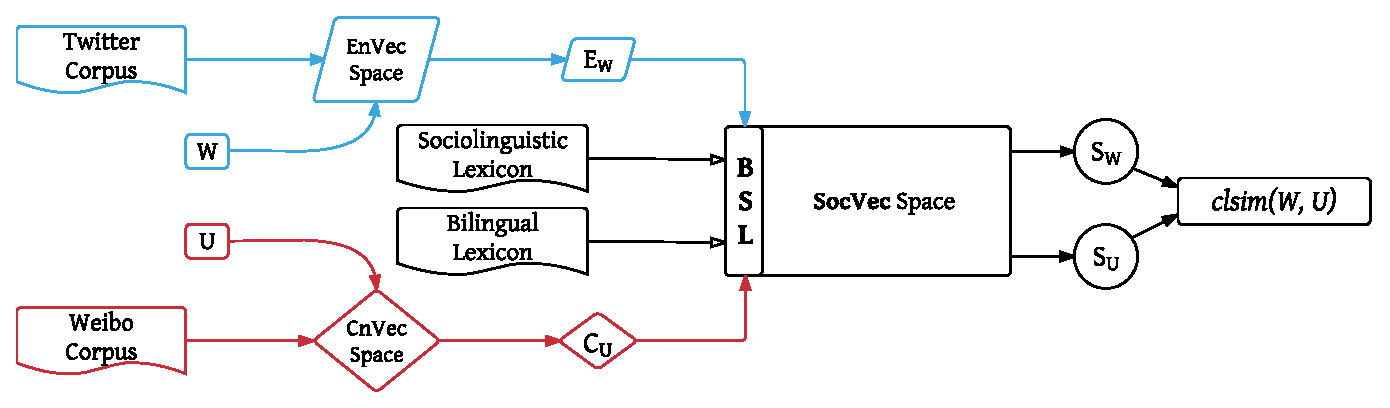
\epsfig{file=overview.pdf, width=1.9\columnwidth}
	\caption{Framework with a LSTM-based classifier}
	\label{fig:LSTM}
\end{figure*}

\subsection{LSTM-based Neural Architectures}
%Although above features are both informative and easy to implement, 
%they involve little sequential information such as the word order.
%LSTMs~\cite{hochreiter1997long} are widely used in relation classification~\cite{socher2011semi,ebrahimi2015chain,xu2015classifying,xu2016improved}.
%capturing not only the input to output but also the sequential relationships.
We observe that the existence of \lnear~relation in 
an instance \textless $s$,$e_1$,$e_2$\textgreater~ depends 
on two major information sources: one is from the semantic and syntactical features of sentence $s$ 
and the other is from the object pair \textless$e_1$,$e_2$\textgreater.
By this intuition, we design our LSTM-based model with two parts, shown in lower part of~\figref{fig:LSTM}.
The left part is for encoding the syntactical and semantic information of the sentence $s$, while the right part is encoding the semantic similarity between the pre-trained word embeddings of $e_1$ and $e_2$.

%\subsubsection{Sentence Normalization}
%A LSTM layer is used to learn the representation of the sentence $s$.
%As for the form of input sentences, 
Solely relying on the original word sequence of a sentence $s$ has two problems:
%(i) the original word sequence concerns little syntactical information;
(i) the irrelevant words in the sentence can introduce noise into the model; 
(ii) the large vocabulary of original sentences induce too many parameters, which may cause over-fitting. For example, given two sentences 
	``\textit{The king led the dog into his nice garden.}'' and 
	``\textit{A criminal led the dog into a poor garden.}''. 
	The object pair is \textless \textit{dog, garden}\textgreater~in 
	both sentences.
	The two words ``\textit{lead}'' and ``\textit{into}'' are essential
	for determining whether the object pair is located near, but they 
are not attached with due importance. 
Also, the semantic differences between irrelevant words, such as ``king'' and ``criminal'', ``beautiful'' and ``poor'', are not useful to the co-location
relation between the ``dog'' and ``garden'', and 
thus tend to act as noise.

\begin{table}[t]
	\centering
%	\small
	\begin{tabular}{l|l}
		\hline
		\textbf{Level}	&  \textbf{Examples}\\ 		\hline
		Objects	& $\textnormal{E}_1$, $\textnormal{E}_2$ \\ 		\hline
		Lemma & open, lead, into, ...\\ \hline 
		Dependency Role	& open\#s, open\#o, into\#o, ... \\ 		\hline 
		POS Tag	& DT, PR, CC, JJ, ... \\ 	\hline 
	\end{tabular}
	\caption{Examples of four types of tokens during sentence normalization. (\#s stands for subjects and \#o for objects)}
	\label{tab:norm}
\end{table}

%To address above issues, we propose utilizing POS (Part-of-Speech) tags instead to capture more syntactical information and reduce the vocabulary size. 
%However, solely doing this loses too much semantic dependency between the words. 
%\textbf{Sentence Normalization.} 
To address the above issues, we propose a normalized sentence representation method merging the three most important and relevant kinds of information about each instance: lemmatized forms, POS (Part-of-Speech) tags and dependency roles. 
We first replace the two nouns in the object pair as ``$\textnormal{E}_1$'' and ``$\textnormal{E}_2$'', and keep the lemmatized form of the original words for all the \textit{verbs, adverbs and prepositions}, which are highly relevant to describing physical scenes.
Then, we replace the \textit{subjects and direct objects} of the \textit{verbs and prepositions} (\texttt{nsubj, dobj} for verbs and \texttt{case} for prepositions in dependency parse trees) with special tokens indicating their dependency roles. 
For the remaining words, we simply use their POS tags to replace the originals. 
The four kinds of tokens are illustrated in ~\tabref{tab:norm}.
\figref{fig:LSTM} shows a real example of our normalized sentence representation, where the object pair of interest is \textless \textit{dog, garden}\textgreater. 
%\begin{table*}[!th]
%	\small
%	\centering
%	\begin{tabular}{lllllllllllll}
%		\hline
%		\textit{The }&\textit{king }&\textit{opened }&\textit{the}&\textit{door}&\textit{and}& \textit{led}& \textit{the}& \textit{\textbf{dog} }& \textit{into }& \textit{his }& \textit{nice }& \textit{\textbf{garden}.}\\		 
%		DT & open\#s & open & DT & open\#o & CC& lead& DT &$\textnormal{E}_1$ & into & PR & JJ& $\textnormal{E}_2$.\\	 \hline
%	\end{tabular}
%	\caption{Sentence Normalization Example}
%	\label{tab:norm_eg}
%\end{table*} 

Apart from the normalized tokens of the original sequence, to capture more structural information, we also encode the distances from each token to $\textnormal E_1$ and $\textnormal E_2$ respectively.
{Such \textit{{position embeddings}} (position/distance features) are proposed by~\cite{zeng2014relation} with the intuition that information needed to determine the relation between two target nouns normally comes from the words which are close to the target nouns.} 

%\subsubsection{Model Training}
%The original sentence is first transformed to normalized sequence described above.

%We adopt this feature because it can help LSTM keep track of the position of $\textnormal E_1$ and $\textnormal E_2$, better knowing \textit{where} the two object words are.
Then, we leverage LSTM to encode the whole sequence of the tokens of normalized representation plus position embedding. 
%\texttt{tanh} activation function is used following~\cite{xu2015classifying}. 
In the meantime, two pretrained \textit{GloVe} word embeddings~\cite{pennington2014glove} of the original two physical object words are fed into a hidden dense layer. 

Finally, we concatenate both outputs and then use \texttt{sigmoid} activation function to obtain the final prediction.
We choose to use the popular binary cross-entropy as our loss function, and
RMSProp as the optimizer. We apply a dropout rate~\cite{zaremba2014recurrent} of 0.5 in the LSTM and embedding layer to prevent overfitting.

\section{\lnear\  Relation Extraction}
\label{sec:mine}
The upper part of \figref{fig:LSTM} shows the overall workflow of our automatic framework to mine LocatedNear relations from raw text.
We first construct a vocabulary of physical objects and generate all candidate instances. 
For each sentence in the corpus, if a pair of physical objects $e_i$ and $e_j$ appear as nouns in a sentence $s$, then we apply our sentence-level relation classifier on this instance. 
The relation classifier yields a probabilistic score $s$
indicating the confidence of the instance in the existence of~\lnear~relation.
Finally, all scores of the instances from the corpus are grouped by the object pairs and aggregated, where each object
pair is associated with a final score. 
These mined physical pairs with scores can easily be integrated into existing commonsense knowledge base.

%\figref{fig:overview} shows the overall workflow of our framework for
%automatic extraction of \lnear\ relationship from text. 
More specifically, for each object pair \textless$e_i,e_j$\textgreater, 
we find all the $m$ sentences in our corpus mentioning both objects.
We classify the $m$ instances with the sentence-level relation classifier and obtain confidence scores for each instance, then
feed them into a heuristic scoring function $f$ to obtain the final aggregated score for the given object pair. 
We propose the following 5 choices of $f$ considering accumulation and threshold:
\begin{align}
	f_0&=m\\
	f_1&=\sum_{k=1}^{m}\textnormal{conf}(s_k,e_i,e_j)\\
	f_2&=\frac{1}{m}\sum_{k=1}^{m}\textnormal{conf}(s_k,e_i,e_j)\\
	f_3&=\sum_{k=1}^{m}1_{\{\textnormal{conf}(s_k,e_i,e_j)>0.5\}} \\
	f_4&=\frac{1}{m}\sum_{k=1}^{m}1_{ \{ \textnormal{conf}(s_k,e_i,e_j)>0.5 \}}
\end{align}
